%---------------------------------------------------------------
\chapter{Background}
%---------------------------------------------------------------

\begin{chapterabstract}
  In this chapter, we introduce the R language and its implementation. We also outline the implementation of Ř, an extension to R which is composed of a bytecode interpreter and a speculative JIT compiler. We compare it to other JIT compilers, namely the V8 for JavaScript and JVM for Java \todo{sync with text}. Finally, we describe the R programs used for experiments and analysis throught the thesis.
\end{chapterabstract}

%------------------------------------------------------------------------------------------------------------------------------
\section{The R Language}
%------------------------------------------------------------------------------------------------------------------------------

\textit{R}\cite{r} is a programming language designed and used for statistical computation, data analysis, and graphical visualization. It was developed Ross Ihaka and Robert Gentleman at the University of Auckland as an alternative to the S language. It is part of the GNU Project, licensed as a free software under GNU GPL.

\begin{figure}[H]
	\centering
	\begin{minipage}{0.45\textwidth}
		\centering
		\begin{minted}{R}
ggplot(
  data = gapminder,
  aes(
    x = gdpPercap, y = lifeExp,
    color = continent
  )
) +
  geom_point() +
  scale_x_log10()
    \end{minted}
		\captionof{listing}{R example\cite{r-crash-course}}\label{lst:motivation}
	\end{minipage}%
	\hfill
	\begin{minipage}{0.45\textwidth}
		\centering
		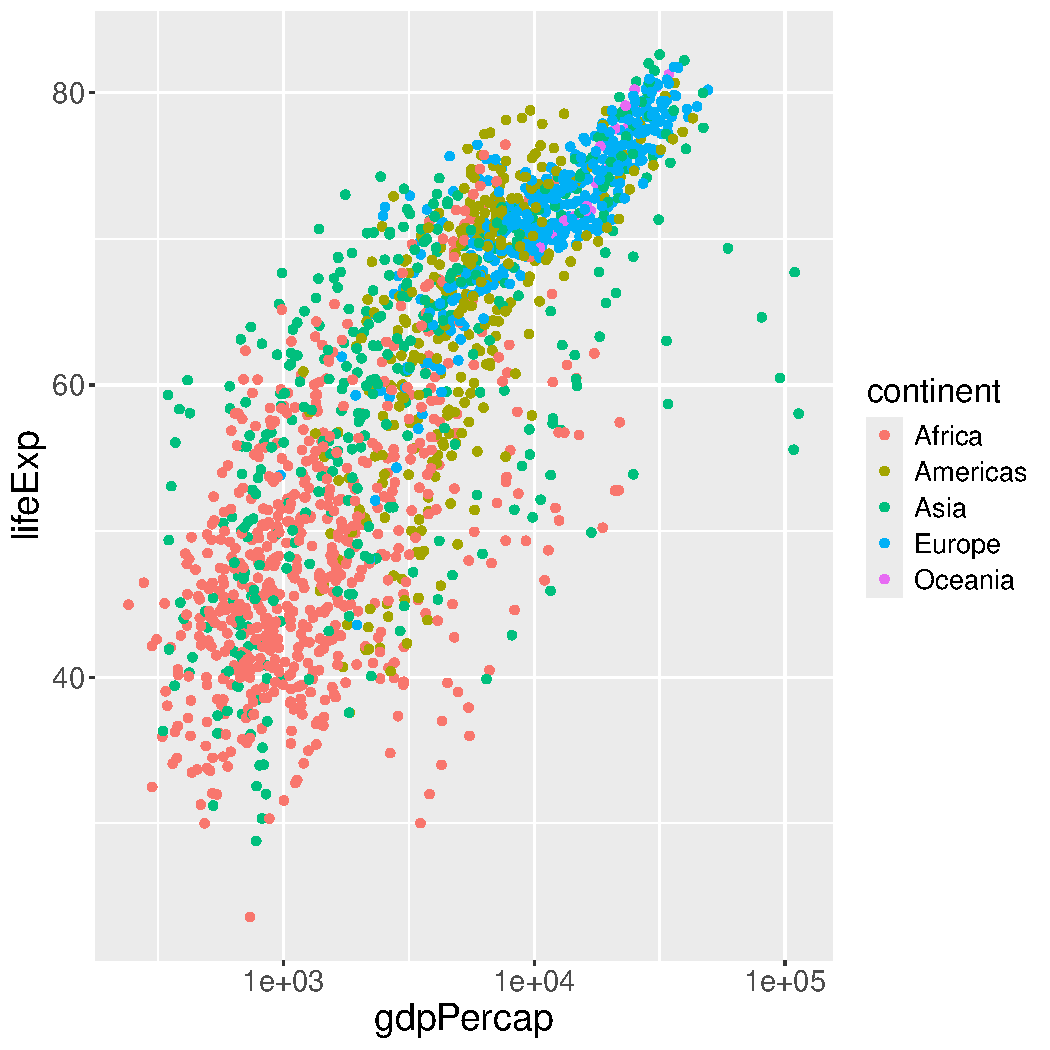
\includegraphics[width=\textwidth]{figures/motivation-Rplots.pdf}
		\caption{Plot of listing \ref{lst:motivation}}
	\end{minipage}
\end{figure}

The popularity of R stems from its domain-specific focus. Unlike general-purpose languages, R offers high-level abstractions for statistical operations, making complex analyses more accessible. As a consequence, many R users users are statisticians rather than traditional programmers. An example of the R expressivity is in the listing \ref{lst:motivation}, where with just a few lines of code we can plot the relationship between the GDP per capita and life expectancy from the \texttt{gapminder} data set\cite{gapminder}.

The language is high-level, dynamic, object-oriented, functional, interpreted, and lazy, with automatic memory management.

The R syntax is very C-like, with \texttt{if} statements, \texttt{for} and \texttt{while} loops, array indexing and function calls. For assignment, the \texttt{<-} operator is used. Statements are separated by newline, optionally by semicolon if they are on the same line.

%---------------------------------------------------------------
\subsubsection*{Types}
%---------------------------------------------------------------

R basic types are the \textit{numeric types} (\textit{integer}, \textit{double} or also \textit{real} and \textit{complex}), \textit{character type} (strings) and \textit{logical type} (the boolean values \texttt{TRUE} and \texttt{FALSE}). R also has \texttt{NULL}, and a constant \texttt{NA} (\textit{not available}) representing a missing value.

R has no concept of scalars. Instead, all basic types are represented as \textit{vectors}. To create a vector with multiple elements, the function \texttt{c} (standing for combine) can be used. All the traditional mathematical operators are also vectorized.

For storing elements of different types, a \textit{list} is used. Other commonly used types built on top of vectors and lists are \textit{matrix} (two-dimensional vector), \textit{array} (multi-dimensional vector) and \textit{data frame} (matrix-like structure whose columns can have different types).

Every type can have associated \textit{attributes}, a collection of name-value pairs. These are accessed via the \texttt{attr} or \texttt{attributes} functions.

R also has multiple \textit{object models}. The most common ones are \textit{S3}, which is controlled by setting a \texttt{class} attribute on any type, and \textit{S4}, which defines more formal classes which have to be created and instantiated, and are internally represnted by a distinct type.

%---------------------------------------------------------------
\subsubsection*{Environments}
%---------------------------------------------------------------

Different scopes in R are separated using objects named \textit{environments}. An environment consists of a \textit{frame}, which is the collection of variables, and a pointer to an \textit{enclosing environment} (also called a \textit{parent}). The topmost environment has a pointer to a special \textit{empty environment}, which has no other parent.

When a variable or a function is accessed, it is first looked for in the current environment. If not found, it is searched for recursively in each enclosing environment. Only then if it is not found, it is an error.

The lookup for functions is separate from non-function lookup. An assignment of a variable in some environment does not shadow a function in its enclosing environment. So the code \texttt{c <- 42; c(c, c)} results in one vector with two numbers 42, because the definition of the variable \texttt{c} does not shadow the function of the same name from the base environment.

These environments are also first-class values. We can create new environments, access the value of the current enclosing environment, or even access and modify environments on the call stack.

%---------------------------------------------------------------
\subsubsection*{Functions}
%---------------------------------------------------------------

A \textit{function}, or also a \textit{closure}, is composed of three parts - \textit{formals}, which is the list of formal arguments and their default values, \textit{body}, which is the code of the function, and \textit{environment} defining the lexical scope of the function body. New functions can be created with the \texttt{function} keyword.

Most operations that happen in R are in fact function calls. This includes the control flow statements (like \textit{if} or \textit{while}), binary operations, assignment, and even surrounding an expression with parenthesis or multiple expression with braces. This is demonstrated in listing \ref{lst:r-special-calls}. Note that built-in functions have to be surrounded with backticks in order to refer to them as identifiers.

\begin{listing}[t]
	\begin{sublisting}[t!]{0.47\textwidth}
		\centering
		\begin{minted}{R}
a <- if (TRUE) {
  1
} else
  2 * (3 + 4)
    \end{minted}
	\end{sublisting}
	\hfill
	\begin{sublisting}[t!]{0.47\textwidth}
		\centering
		\begin{minted}{R}
# This is equivalent to
# the previous statement
`<-`(a, `if`(
  TRUE,
  `{`(1),
  `*`(
    2,
    `(`(`+`(3, 4))
  )
))
    \end{minted}
	\end{sublisting}
	\caption{Demonstration of R special calls}\label{lst:r-special-calls}
\end{listing}

%---------------------------------------------------------------
\subsubsection*{Laziness}
%---------------------------------------------------------------

R is lazy in arguments. This means that when a function is called, the passed arguments are not instantly evaluated, but are instead wrapped in a \textit{promise}, a tuple of \textit{expression}, \textit{value}, and \textit{environment}. The value is at first set to the unbound value. When the promise is first accessed, the expression of the promise is evaluated within its environment (also called a \textit{force}). The result is cached in the value field, and every other access to the argument results in the cached value.

This can be seen in example \ref{lst:example-lazy}. The call at line 12 first prints \enquote{Hello from g}, then the parameter \texttt{x} is accessed, the promise is forced, and the text \enquote{Hello from f} is printed. The second call to the function \texttt{h} demonstrates a second behavior - when a parameter is never accessed, the promise is not evaluated, and nothing is printed.

\begin{listing}[h!]
	\centering
	\begin{minted}{R}
f <- function(x) {
    print("Hello from f")
    x
}

g <- function(x) {
    print("Hello from g")
    x
}

# Prints "Hello from g", then "Hello from f"
g(f(42))

h <- function(x) 0

# Does not print anything
h(f(42))
  \end{minted}
	\caption{Example of R laziness}\label{lst:example-lazy}
\end{listing}

Being lazy in the arguments allows R to have very expressive domain-specific languages for ease of manipulating the data, as well as reducing memory overhead of the programs.

Promises can also be created manually by calling the \texttt{delayedAssign} function or from the C API.

%---------------------------------------------------------------
\subsubsection*{Immutability}
%---------------------------------------------------------------

All R values are \textit{semantically immutable}, with the exception of environments. This means that when a variable holds a value, this value never changes unless the variable is reassigned. We say that non-environment values have a \textit{copy-on-write behavior} - when a value is modified, a new copy is created with the modified parts.

Thanks to the syntax of R, it is possible to write code that looks like it is using mutability, but keeps the copy-on-write behavior. In the example \ref{lst:imm}, the statement on line 3 looks like it is mutating the vector in place, but instead the function \texttt{[<-} is called, which creates a copy of the vector, modifies it and reassigns the variable x.

The only truly mutable values are environments, and they conform to a \textit{reference behavior}. Listing \ref{lst:envir} shows this behavior - the variable \texttt{x} is added to both \texttt{e1} and \texttt{e1}, even though we only defined it on \texttt{e2}.

\begin{listing}
	\centering
	\begin{minipage}{0.47\textwidth}
		\begin{minted}{R}
x <- c(1, 2, 3)
y <- x
y[1] <- 42
# x is still vector (1, 2, 3)
      \end{minted}
		\caption{Immutability example}\label{lst:imm}
	\end{minipage}
	\hfill
	\begin{minipage}{0.47\textwidth}
		\begin{minted}{R}
e1 <- new.env()
e2 <- e1
e2$x <- 42
e1$x == 42
# TRUE
      \end{minted}
		\caption{Example of environment mutability}\label{lst:envir}
	\end{minipage}
\end{listing}

%---------------------------------------------------------------
\subsubsection*{Reflection}
%---------------------------------------------------------------

As mentioned before, environments are a first-class citizen. This allows for any function to access and even modify any environment where it was created or called. Moreover, when combined with lazy arguments, a function can reflect on the environment it is being forced in and modify it, sometimes in unpredictable ways.

This is demonstrated in listing \ref{lst:bad-ref}. We can see that evaluating the promise (the call to \texttt{bad}) removes a variable binding, resulting in an error.

\begin{listing}
	\centering
	\begin{minted}{R}
bad <- function() {
  rm("x", envir=sys.frame(-1)) # Remove the variable x from the caller
  2
}

good <- function(y) {
  x <- 1
  z <- y # Here the promise is evalated
  x + z
}

good(bad())
# Error in good(bad()) : object 'x' not found
  \end{minted}
	\caption{Example of malicious reflection\cite{r-melts-brains}}\label{lst:bad-ref}
\end{listing}

R also has primitives for creating, manipulating, and evaluating expressions from the language itself. This allows for, among other things, evaluating a promise under a different environment, programatically creating arbitrary pieces of code, or instrumenting functions with additional calls.

Combining reflection, laziness and side effects makes R a very complex language to optimize.

\newpage
%------------------------------------------------------------------------------------------------------------------------------
\section{GNU-R}
%------------------------------------------------------------------------------------------------------------------------------

The R language is not formally specified, it only has a reference implementation that we will refer to as \textit{GNU-R}. It is written in the C programming language, spans over more than {250 000} lines of code and is currently maintained by the R Core Team

%---------------------------------------------------------------
\subsubsection*{Representation}
%---------------------------------------------------------------

The GNU-R represents all code and values as \textit{symbolic expressions} (also \textit{S-expressions} or \textit{SEXPs}), a format for nested lists popularized by the Lisp languages. The type \texttt{SEXP} is a pointer to either a \texttt{SEXPREC} or \texttt{VECTOR\_SEXPREC} structure. Both of these structures contain a header of type \texttt{sxpinfo\_struct}, a pointer to the attributes list, and previous and next nodes in the garbage collector. The \texttt{sxpinfo\_struct} then contains \texttt{SEXPTYPE}, the type of the SEXP (values are defined as in \ref{tbl:sexptype}), as well as additional information about the type, garbage collection and debug informations. The rest of the structure cointains the actual data. The structure of a \texttt{SEXP} value is represented in figure \ref{fig:sexp-struct}.

As a note, throught the thesis, when referring to a SEXP value, we do mean the actual behind the \texttt{SEXP} pointer.

\begin{figure}
	\centering
	\begin{adjustbox}{trim=5pt 20pt 0 40pt, clip}
		\includediagram{0}
	\end{adjustbox}
	\caption{Structure of the GNU-R \texttt{SEXP} type}\label{fig:sexp-struct}
\end{figure}

\begin{table}[h!]
	\centering
	\begin{tabular}{c l l}
		\hline
		\textbf{no} & \textbf{SEXPTYPE} & \textbf{Description}       \\
		\hline
		0           & NILSXP            & NULL                       \\
		1           & SYMSXP            & symbols                    \\
		2           & LISTSXP           & pairlists                  \\
		3           & CLOSXP            & closures                   \\
		4           & ENVSXP            & environments               \\
		5           & PROMSXP           & promises                   \\
		6           & LANGSXP           & language objects           \\
		7           & SPECIALSXP        & special functions          \\
		8           & BUILTINSXP        & builtin functions          \\
		9           & CHARSXP           & internal character strings \\
		10          & LGLSXP            & logical vectors            \\
		13          & INTSXP            & integer vectors            \\
		14          & REALSXP           & numeric vectors            \\
		15          & CPLXSXP           & complex vectors            \\
		16          & STRSXP            & character vectors          \\
		17          & DOTSXP            & dot-dot-dot object         \\
		18          & ANYSXP            & make “any” args work       \\
		19          & VECSXP            & list (generic vector)      \\
		20          & EXPRSXP           & expression vector          \\
		21          & BCODESXP          & byte code                  \\
		22          & EXTPTRSXP         & external pointer           \\
		23          & WEAKREFSXP        & weak reference             \\
		24          & RAWSXP            & raw vector                 \\
		25          & OBJSXP            & objects not of simple type \\
		\hline
	\end{tabular}
	\caption{The different SEXP types\cite[1.1.1 SEXPTYPEs]{rprojectInternals}}\label{tbl:sexptype}
\end{table}

%---------------------------------------------------------------
\subsubsection*{Interpreter}
%---------------------------------------------------------------

The GNU-R parses the code into an \textit{abstract syntaxt tree} (\textit{AST}), represented by SEXPs of the \texttt{LANGSXP} type, which is then interpreted.

Included with the distribution of GNU-R is a \textit{bytecode compiler}, which can be invoked either explicitly, when a package is installed, or as a just-in-time (JIT) compiler. The compiler is written mostly in R with few supporting functions written in C, while the bytecode interpreter is written in C. The bytecode is stack-based with fat instructions, like specialized instructions for type checking, specialized loads for common constants like \texttt{NULL}, \texttt{TRUE} or \texttt{FALSE}, instructions for executing \texttt{for} loops or various subsetting operators. Branching is done via jumps to arbitrary code index. An example of the bytecode can be seen in listing \ref{lst:bc-example-gnur}.

The bytecode employs a series of optimizations, most notably constant folding and inlining of base and builtin functions. The inlining can be set to various levels, with higher levels being more optimized while assuming that the functions in the base package and core language functions (like \texttt{if} or \texttt{`\{`}) are not shadowed. This allows the compiler to translate control flow from function calls to bytecode jumps, as well as to use bytecode instructions to perform basic arithmetic and logical operations.

When a function is compiled, its \texttt{SEXP} is modified in-place, replacing the AST body with a bytecode. Every other call to this function is then interpreted by the bytecode interpreter, which is written in C and is also is part of the GNU-R.

\begin{listing}[p]
	\centering
	\begin{minipage}{0.33\textwidth}
    \begin{minted}[fontsize=\small,linenos=false]{R}
f <- function(x) {
  for (i in 1:10) {
    if (i + 2 > 1) {
      g(x)
    }
  }
  g(x)
}
    \end{minted}
		\subcaption{R code}\label{lst:bc-example-r}
	\end{minipage}
	\hfill
	\begin{minipage}{0.66\textwidth}
		\begin{minipage}{0.20\textwidth}
			\begin{minted}[fontsize=\small,linenos=false]{text}
Code:
  1 LDCONST 1
  3 STARTFOR 4 3 30
  7 GETVAR 3
  9 LDCONST 5
 11 ADD 6
 13 LDCONST 7
 15 GT 8
 17 BRIFNOT 9 28
 20 GETFUN 10
 22 MAKEPROM 12
 24 CALL 11
 26 GOTO 29
 28 LDNULL
 29 POP
 30 STEPFOR 7
 32 ENDFOR
 33 POP
 34 GETFUN 10
 36 MAKEPROM 12
 38 CALL 11
 40 RETURN
      \end{minted}
		\end{minipage}
		\hfill
		\begin{minipage}{0.48\textwidth}
			\begin{minted}[fontsize=\small,linenos=false]{text}
Constant pool:
0:
 language {  for (i in 1:10) {; i..
1:
 int [1:10] 1 2 3 4 5 6 7 8 9 10
2:
 language 1:10
...
12:
 Promise 0:
  Code:
    1 GETVAR 0
    3 RETURN
  Constant pool:
  0:
   symbol x
  1:
   language g(x)
  2:
   'expressionsIndex' int [1:4] N..
13:
 'expressionsIndex' int [1:41] NA..
      \end{minted}
		\end{minipage}
		\subcaption{GNU-R code}\label{lst:bc-example-gnur}
	\end{minipage}
	\par\vspace{2mm}\par
	\begin{minipage}{\textwidth}
		\centering
		\begin{minipage}{0.47\textwidth}
			\begin{minted}[fontsize=\small,linenos=false]{\rirlexer}
0:
      0   push_  1
      5   visible_
      6   force_
      7   push_  10
     12   visible_
     13   force_
     14   ; :(1, 10)
          colon_input_effects_
     15   pop_
     16   swap_
     17   colon_cast_lhs_
     18   [ <?> ] Type#0
     23   ensure_named_
     24   swap_
     25   colon_cast_rhs_
     26   ensure_named_
     27   [ <?> ] Type#1
     32   dup2_
     33   ; NULL
          le_
     34   [ _ ] Test#0
     39   brfalse_  1
     44   push_  1L
     49   br_  2
      \end{minted}
		\end{minipage}
		\hfill
		\begin{minipage}{0.47\textwidth}
			\begin{minted}[fontsize=\small,linenos=false]{\rirlexer}
1:
     54   push_  -1L
     ...
7:
    287   popn_  3
    292   ldfun_  g
    297   [ 0, <0>, valid  ] Call#2
    302   mk_promise_  2
    307   ; g(x)
          call_  1
    324   [ <?> ] Type#11
    329   ret_

[Prom (index 0)]
0:
      0   ldvar_  x
      5   [ <?> ] Type#5
     10   ret_

[Prom (index 1)]
0:
      0   ldvar_  x
      5   [ <?> ] Type#9
     10   ret_
     ...
      \end{minted}
		\end{minipage}
		\subcaption{RIR code}\label{lst:bc-example-rir}
	\end{minipage}
  \caption{A truncated example of generated GNU-R and RIR bytecodes, full code in appendix \todoadd}\label{lst:bc-example}
% \ref{ch:appendix-bc}
\end{listing}


%---------------------------------------------------------------
\subsubsection*{Garbage Collector}
%---------------------------------------------------------------
R does not have primitives for managing memory, instead an automatic memory management provided by the runtime is expected. GNU-R uses a generational non-moving stop-the-world garbage collector with three generations\cite{r-gc-notes}.

Next to the GC, GNU-R also has a reference counter for each object, included in the object header. This is used for optimistic mutations---when an object would be copied and mutated, but there is only one reference to it, it is instead mutated in place, avoiding unnecesarry copies. This correctly preserves the copy-on-write behavior while improving performance.

%---------------------------------------------------------------
\subsubsection*{Packages}
%---------------------------------------------------------------

A big advantage of using R is the vast library of packages, libraries and data sets. These are hosted at \textit{The Comprehensive R Archive Network} (\textit{CRAN})\cite{cran} package repository, wich is currated and tested by the R Core Team. They can be very simply installed by calling \texttt{install.packages} and loaded with the \texttt{library} function.

The GNU-R base installation is also distributes with several packages, including, but not limited to, \texttt{base} containing the basic functions for using R, \texttt{stats} implementing statistical functions, \texttt{graphics} with base functions for manipulating graphical output, \texttt{compiler} implementing the mentioned bytecode compiler, or \texttt{Matrix} with definitions of dense and sparse matrix classes.

%---------------------------------------------------------------
\subsubsection*{C Interface}
%---------------------------------------------------------------

In order to speed-up certain packages, GNU-R allows parts of the code to be written in more low-level languages via a C interface. This includes the definitions for the SEXP types, a big set of functions and macros to create and manipulate values, as well as several evaluations functions. The SEXP structure is only exported as an opaque pointer, with the intent that individual fields are to be accessed and manipulated via the exported functions.

The interface is more of an after thought more than a deliberate choice, as indicated for example by the the main file with type definitions being called \texttt{Rinternals}. The functions expose big portion of the internal structure and this is subsequently used by package authors. Even parts of the code that are not directly exposed are commonly accessed by packages. As an example, some packages rely on the hidden reference counter in order to optimize updates by modifying structures in-place.

This makes evolution of R without breaking packages very hard, as well as complicating alternative implementations of R as they need to explicitly export the same functions as GNU-R if they want to support all available libraries.

\newpage
%------------------------------------------------------------------------------------------------------------------------------
\section{The Ř Compiler}
%------------------------------------------------------------------------------------------------------------------------------

\textit{Ř} (also stylized as \textit{Rsh}) is a just-in-time compiler for the R language, developed at Programming Languages Laboratory at Czech Technical University in Prague\footnote{\url{https://prl-prg.github.io/}} and Programming Research Laboratory at Notheastern University in Boston\footnote{\url{https://prl.khoury.northeastern.edu/}}. The project is freely available and hosted on GitHub\cite{rsh-github}.

It is built as an extension to GNU-R, although it uses a slightly modified version of the codebase. It bypasses the GNU-R bytecode compiler and interpreter, instead using a custom one, while reusing the \texttt{SEXP} representation, AST interpreter, and garbage collector. For the compilation to native code, the \textit{LLVM Project}\cite{llvm} is used. The compilation pipeline is outlined in figure \ref{fig:rsh-archit}

\begin{figure}
	\centering
	\includediagram[0.7]{3}
	\caption{Overview of Ř architecture\cite{reusing-jit}}\label{fig:rsh-archit}
\end{figure}

%---------------------------------------------------------------
\subsubsection*{Runtime Objects}
%-------------------------------------------------------------
Ř reuses SEXP representation and memory management from GNU-R. All runtime objects are embedded into the SEXP objects. This is one of the modifications that need to be applied to GNU-R, a new \texttt{SEXPTYPE} is added (\texttt{EXTERNALSXP}), along with the necessary changes to how it is garbage collected and how it references other objects.

The structure of Ř runtime object can be seen in figure \ref{fig:rsh-object-struct}. It contains the \texttt{SEXP} header of the \texttt{EXTERNALSXP} type, and then the embeded Ř object, which always inherit from a \texttt{RirRuntimeObject} class. The Ř object always starts with two \texttt{uint32\_t} numbers, the first dictates how many bytes after the start of the object is the begining of area referencing other SEXPs, and the second indicates how many pointers are there. The magic number dictates which Ř object it is.

There are helpers macros to access the headers, as well as the pointers to other \texttt{SEXP}s. On the Ř side, there are functions to convert between a C++ pointer and a SEXP.

\begin{figure}
	\centering
	\begin{adjustbox}{trim=10 80pt 0 0, clip}
		\includediagram{1}
	\end{adjustbox}
	\caption{Structure of the Ř runtime objects}\label{fig:rsh-object-struct}
\end{figure}

Similarly to the GNU-R compiler, when an R function is to be interpreted, it is compiled to a bytecode, and the body field of the closure is instead replaced by a Ř structure. The composition of Ř objects can be seen in figure \ref{fig:rsh-composition}.

The body of Ř compiled function contains a \textit{dispatch table}. A dispatch table contains multiple entries of compiled code, where the first version (also called a \textit{baseline}) is always the bytecode representation, whereas the other versions are compiled to native code. Each native entry corresponds to one version compiled under a unique call context, as used by the contextual dispatch (explained in chapter \ref{ch:1-ctx-dispatch}).

Every dispatch table entry is represented by a \texttt{Function} structure. This holds the signature of the function, the call context, statistic about the execution like how many times it has been invoked or deopted, the body of the function and the feedback vector.

The body of a function is stored in a structure called \texttt{Code}. This is either the bytecode body or a pointer to the native function, and the constants pool.

The \textit{feedback vector} collected from a bytecode interpretation is represented by the \texttt{TypeFeedback} structure\footnote{\texttt{TypeFeedback} is a missleading name as the interpreter also collect non-type information}. It consists of \textit{slots}, where one slot corresponds to information about one bytecode instruction. There are three different types of slots:
\begin{itemize}
  \item{} \textit{observed calls} records the destination of calling a function,
  \item{} \textit{observed types} record the types of values that are loaded from environment, forced, or are results of a function call,
  \item{} and \textit{observed tests} has one of four values recording how a branch was taken (\texttt{None}, \texttt{OnlyFalse}, \texttt{OnlyTrue} and \texttt{Both}).
\end{itemize}
Since every function has different number of slots, the \texttt{TypeFeedback} object has different size for each function and is using a \textit{flexible array member}\cite{flexible-array} to store the observations.

\begin{figure}
	\centering
	\includediagram[0.7]{2}
	\caption{Composition of Ř runtime objects}\label{fig:rsh-composition}
\end{figure}

%---------------------------------------------------------------
\subsubsection*{RIR Bytecode Interpreter}
%---------------------------------------------------------------

The bytecode used by Ř is called \textit{RIR}. It is a stack-based bytecode, interpreted by a Ř interpreter. Similarly to GNU-R, RIR assume the base functions are not shadowed, allowing it to have instrucitons for arithmetic operations and control flow instead of resolving them as function calls. Unlike GNU-R, the RIR instructions are much more granular, there are fewer of them, they are not as specialized and a single instruction represent much smaller piece of C code. An example of RIR compiled code can be seen in listing \ref{lst:bc-example-rir}. Note that the example code is not complete and is only used to give impression between the size differences of the bytecodes and the full code listing is in appendix \ref{ch:appendix-bc}.

For this thesis, the important bytecode instructions are \texttt{record\_call\_}, \texttt{record\_type\_}, and \texttt{record\_test\_}. These do the recording of feedback information about calls, types and tests respectively by observing the top value on the execution stack and recording the information to the \texttt{TypeFeedback} structure on an index stored as an immediate value. The instructions are printed in listings as the current feedback value in square brackets followed by the label \texttt{Call\#N}, \texttt{Type\#N} or \texttt{Test\#N}, where \texttt{N} is the slot index.

Apart from the feedback information, the RIR interpreter also records other informations about the running program, most notably the number of times a function has been invoked, and the number of times a loop has been executed. These are used to determine which parts of the program are executed frequently, and thus are a good candidates for compiling to native code.

%---------------------------------------------------------------
\subsubsection*{PIR Compiler}
%---------------------------------------------------------------

When a function or a loop meets the compilation heuristics, it is compiled from RIR to \textit{PIR}, an intermediate representation used for optimizations. PIR is composed of instructions in a \textit{static single-assignment form} (SSA), organized in basic blocks, with each block being terminated with a (conditional) jump to another basic block, or a speculation checkpoint.

Every PIR instruction has a \textit{type} (also called a \textit{PIR type}). These consist of one or several \textit{R types} (like integer or logical) and type flags. For this thesis, the important type flags are
\begin{itemize}
	\item{} \textit{is scalar}, meaning the value is always a vector of size 1,
	\item{} \textit{is not object}, which means that the value is neither of the R object models,
	\item{} \textit{has no attributes}, where the object does not have the associated R attributes (this implies it is not an object),
	\item{} \textit{can be missing}, where the value can be an \textit{unbound value}, raising an error if evaluated,
	\item{} \textit{can be NA or NaN}, meaning the value can be \texttt{NA} or a not-a-number (NaN),
	\item{} and \textit{maybe lazy}, where the value needs to be first evaluated before used.
\end{itemize}
All of these types form a complete lattice. There are also types which model the types internal to only the PIR code, used for the speculative optimizations.

All of the instructions also have a \textit{effect flags}, denoting what kind of observable side effects an instruction can emit. These for example include \textit{deopt} (may trigger deoptimization), \textit{warn} (might print a warning messages respectively), \textit{error} (might produce an error), or \textit{reflection} (might invoke reflection). By explicitly tracking these effect the compiler is are able to perform more optimizations while still preserving the correct R semantics.

In listing \ref{lst:instruction-example}, we can see the how the PIR instructions are represented in text. It starts with the type (\texttt{real\$-}), continues with the register by which the instruciton is referred to (\texttt{\%4.2}), then the name of instruction (\texttt{Add}), followed by effect flags (\texttt{d}), arguments (\texttt{\%2.0, 2, elided}) and finally the feedback slot connected with this instruction (\texttt{<val?\_>}). When the type of instruciton is void, the register is ommited. Similarly, when the instruction does not have a feedback connected with it, it is not shown.

\begin{listing}[H]
  \begin{minted}[linenos=false]{\pirlexer}
real$-    %4.2 = Add     d     2.0, 2, elided     <val?_>
  \end{minted}
	\caption{Example of a PIR instruction}\label{lst:instruction-example}
\end{listing}

Based on the observed feedback, the compiler performs \textit{speculative optimizations}. When the feedback slot on a PIR instruction hold interesting information (e.g. the callee is only one target, branch was always taken or the observed type was a only integer), Ř \textit{speculates} on this observation. It emits a \textit{guard} which will assert at runtime that the speculation still holds and the rest of the code uses the speculation as a given fact. After the compilation, if the guard fails, a \textit{deoptimization} is triggered. This updates the feedback slot with the newly observed fact, marks the native code version with a flag, and continues execution in the bytecode interpreted version. A \textit{frame state} is used to reconstruct the environment and execution stack to a corresponding state for the interpreter to correctly continue execution.

After all of the optimizations are finished, the PIR code is transformed into \textit{LLVM bitcode}, the intermediate representation of LLVM. This is then passed to the \textit{ORC JIT} compiler, which is part of the LLVM project, compiling the bitcode to the native code.

%---------------------------------------------------------------
\subsubsection*{Contextual Dispatch}\label{ch:1-ctx-dispatch}
%---------------------------------------------------------------

Next to the speculative optimizations, Ř employs another technique for optimizing on dynamic types called \textit{contextual dispatch}\cite{ctx-dispatch}. The idea is based on observing arguments on runtime and based on their types, creating a disjunct native version with the ability to specialize uniquely to the type.

For every function call, we can create a \textit{context}. It captures information about the first six arguments (if they are eager, non-reflective, not an object, or a simple scalar integer or double), the number of missing arguments, as well as if the arguments are correctly ordered, or if there is not too many arguments passed. These contexts form a partial ordering.

When a function compilation to native is triggered, it is compiled for a specific context and the compiler is able to optimize on the information in the context. The resulting code with the context (together called a \textit{version}) is installed into the dispatch table.

When a function is invoked, its arguments are observed and a call context is created. Based on this, the function is either dispatched to the version connected with the same context as the call context, or a less precise context which is ordered lower than the call context. If no such version is found, the call is dispatched to the baseline interpreted version.

%---------------------------------------------------------------
\section{Corpus}\label{ch:1-corpus}
%---------------------------------------------------------------

For the experiments and analysis, we use two codebases.

The first one is a collection of Ř benchmarks\footnote{\url{https://github.com/reactorlabs/RBenchmarking}}. This consists of four different suites of benchmarks:
\begin{itemize}
	\item{} \textit{Are We Fast Yet}, a collection of both micro and macro benchmarks based on the cross-language compiler benchmark suite\cite{are-we-fast-yet},
	\item{} \textit{Real Thing}, a collection of real-world programs,
	\item{} \textit{Shootout} benchmarks from a popular cross-language benchmarks game\cite{shootout},
	\item{} and \textit{Simple}, which are custom written short scripts used for microbenchmarking individual R features.
\end{itemize}

The second codebase is a script from a Kaggle competition about machine learning on the Titanic dataset\cite{titanic}. This script was chosen as a representatn of a more more real-world program. It contains 108 lines of code extracted from a Rmarkdown notebook, and uses some of the most popular R libraries like \texttt{ggplot2} or \texttt{dplyr}.

%---------------------------------------------------------------
\section{Related Work}
%---------------------------------------------------------------

We want to compare how feedback is collected in other VMs. \todoadd

It is a state of of the art JavaScript virtual machine.

%---------------------------------------------------------------
\subsubsection*{V8}
%---------------------------------------------------------------

V8\todocite is the JavaScript and WebAssembly engine developed by Google and used in the Chrome web browser.

The V8 compilation is split into four different stages---a profiling bytecode compiler (Ignition), a non-optimizing profiling JIT compiler (Sparkplug) and two non-profiling optimizing JIT compilers (Maglev and TurboFan).

In the profiling stages, V8 collects the information about the shapes of dynamic JavaScript objects called \textit{maps}. These describe the layout of objects like on which offset is a field stored. This information is recored in an \textit{inline cache} (\textit{IC}) for each load and store. Appart from being used as a feedback, inline caches also speed up the interpreted instructions. All inline caches are stored per function in a \textit{feedback vector}.

An initialized inline cache can be in one of three states -- \textit{monomorphic} meaning only one object shape was observed, \textit{polymorphic} if multiple object shapes were observed, and \textit{megamorphic} where too many object shapes were observed and the inline cache is degraded.

When optimizing, V8 speculates on these inline caches. If the IC is monomorphic, it guards that the actual object has the expected shape. If is is polymorphic, it generates an equivalent of a switch statement on the observed maps, where on failure to match it deoptimizes. V8 compilers do not speculate on megamorphic ICs.

Contrary to Ř, V8 does not speculate eagerly, i.e. whenever the feedback information allows it, but only when the information is used. So for example while compiling the JavaScript function

\mintoneline{js}{function f(a, b) { return a + b }}

\noindent it only assumes on the arguments \texttt{a} and \texttt{b} when compiling the plus operator.

%---------------------------------------------------------------
\subsubsection*{HotSpot}
%---------------------------------------------------------------

HotSpot is a Java Virtual Machine (JVM) currently developed by Oracle. It uses five-tiered architecture.
